\documentclass[12pt, a4paper, portrait]{report}

%packages
\usepackage[german]{babel}
\usepackage[utf8]{inputenc}
\usepackage{graphicx}
\usepackage{amsmath}
\usepackage{amssymb}
\usepackage{anysize}
\usepackage{titlesec}
\usepackage{gensymb}
\usepackage{trfsigns}
\usepackage{multirow}
\usepackage{xcolor}
\usepackage{geometry}
\usepackage{float}
\usepackage{svg}
\usepackage{pdflscape}
\usepackage{rotating}
\usepackage{enumitem}
\usepackage{datetime}
\usepackage[onehalfspacing]{setspace}
\usepackage[backend=bibtex, style=alphabetic]{biblatex}
\usepackage{siunitx}
\usepackage{textpos}
\usepackage{fancyhdr}
\usepackage{lastpage}
\usepackage{listings}
\usepackage{courier}

\addbibresource{literature/bibliographie.bib}

\newcounter{UseCaseNumber}
\setcounter{UseCaseNumber}{1}

\newcommand{\usecaseSmall}[2]{
	\subsection*{Anwendungsfall \arabic{UseCaseNumber}: #1}
	\begin{tabular}{|p{6cm}|p{18.5cm}|}
		\hline
		Name & #1 \\
		\hline
		Kurzbeschreibung & #2 \\
		\hline
	\end{tabular}
	\stepcounter{UseCaseNumber}
}

\newcommand{\usecaseBigA}[6]{%
	\def\usecaseArgA{#1}%
	\def\usecaseArgB{#2}%
	\def\usecaseArgC{#3}%
	\def\usecaseArgD{#4}%
	\def\usecaseArgE{#5}%
	\def\usecaseArgF{#6}%
}

\newcommand{\usecaseBigB}[6]{
	\subsection*{Anwendungsfall \arabic{UseCaseNumber}: \usecaseArgA}
	\begin{tabular}{|p{6cm}|p{18.5cm}|}
		\hline
		Name & \usecaseArgA \\
		\hline
		Kurzbeschreibung & \usecaseArgB \\
		\hline
		fachliches Ziel & \usecaseArgC \\
		\hline
		Akteure & \usecaseArgD \\
		\hline
		Auslöser & \usecaseArgE \\
		\hline
		Vorbedingung & \usecaseArgF \\
		\hline
		Nachbedingung & #1 \\
		\hline
		verwendete Informationen & #2 \\
		\hline
		Ergebnis & #3 \\
		\hline
		Ablauf & #4 \\
		\hline
		Abläufe in Ausnahmefällen & #5 \\
		\hline
		Verweise & #6 \\
		\hline
	\end{tabular}
	\stepcounter{UseCaseNumber}
}
% format before document start

\geometry{
	a4paper,
	left=25mm,
	right=25mm,
	top=25mm,
	bottom=30mm,
	footskip=5mm
	}

% global text font
\renewcommand{\familydefault}{lmss}

%turn of page numbering
\pagenumbering{gobble}

% prevent single lines on top or bottom of page
\widowpenalty = 10000
\clubpenalty = 10000

% spaces
\setlength{\parskip}{2pt} % space after praragraph
\setlist{noitemsep, topsep=3pt} % space before and between enumerations, item lists



% spave before and after equations. Does not do anything yet
\setlength{\abovedisplayskip}{0pt}
\setlength{\belowdisplayskip}{0pt}
\setlength{\abovedisplayshortskip}{0pt}
\setlength{\belowdisplayshortskip}{0pt}

% listings
\lstset{frame=single, firstline=1, numbers=left, numberstyle=\small, basicstyle=\small\ttfamily, captionpos=b, belowskip=-0.5 \baselineskip}


\renewcommand{\lstlistingname}{Quellcode}
\renewcommand{\lstlistlistingname}{Quellcodeverzeichnis}

% formats for headings
\titleformat{\chapter}
{\normalfont\LARGE\bfseries}{\thechapter.}{16pt}{}
%\titlespacing{\chapter}{0pt}{-35pt}{10pt}
\titlespacing{\chapter}{0pt}{-20pt}{10pt}

\titleformat{\section}
{\normalfont\Large\bfseries}{\thesection}{14pt}{}
\titlespacing{\section}{0pt}{10pt}{5pt}

\titleformat{\subsection}
{\normalfont\normalsize\bfseries}{\thesubsection}{12pt}{}
\titlespacing{\subsection}{0pt}{10pt}{10pt}

\titleformat{\subsubsection}
{\normalfont\normalsize\bfseries}{\thesubsubsection}{12pt}{}
\titlespacing{\subsubsection}{0pt}{10pt}{10pt}

\titleformat{\paragraph}[runin]
{\normalfont\normalsize\bfseries}{\theparagraph}{12pt}{}
\titlespacing{\paragraph}{0pt}{10pt}{5pt}

\titleformat{\subparagraph}[runin]
{\normalfont\normalsize\bfseries}{\thesubparagraph}{12pt}{}
\titlespacing{\subparagraph}{\parindent}{10pt}{5pt}

\pagenumbering{arabic}

\newdateformat{dateGerman}{\twodigit{\THEDAY}.\twodigit{\THEMONTH}.\THEYEAR}

\renewcommand{\baselinestretch}{1.5} 

% HEADER and FOOTER

\newcommand{\kopfzeile}{Personalentwicklung und Ausbildung Feuerbach \\ Technische Studiengänge an der DHBW}

\newcommand{\fusszeile}{PEA3-Fe - betriebliche Ausbildung technische Studiengänge der DHBW  \\ \copyright \text{ }Alle Rechte bei der Robert Bosch GmbH, auch für den Fall von Schutzrechtsanmeldungen. Jede Verfügungsbefugnis, wie Kopier- und Weitergaberecht bei uns.}

\pagestyle{fancy}
\renewcommand{\headrulewidth}{0.5pt}
\renewcommand{\footrulewidth}{0.5pt}

%this command set the header and footer to the style of the first few pages
\newcommand{\fancyhfStyleOpening}[0]{
	
	% current style
	\fancyhf{}
	\fancyhead[L]{\small \kopfzeile}
	\fancyhead[R]{
		\begin{textblock*}{4.0cm}(78.0mm, -8.0mm)
			
\includegraphics[height=1.1cm]{resources/logos/DHBW-Logo.png}
		\end{textblock*}
		\begin{textblock*}{4.0cm}(120.0mm, -16.0mm)
			
\includegraphics[height=2.0cm]{resources/logos/Bosch-Logo-Kopfzeile.png}
		\end{textblock*}
	}
	\fancyfoot[L]{
		\tiny \fusszeile
		\vspace{2mm}
		\begin{tabular*}{16cm}{@{\extracolsep{\fill}}l>{
					\raggedleft}p{8cm}}
			{\small Stand: \today} & 
			{\small Seite \thepage}
		\end{tabular*}
	}
	
	% default stlye
	\fancypagestyle{plain}{
		\fancyhf{}
		\fancyhead[L]{\small \kopfzeile}
		\fancyhead[R]{
			\begin{textblock*}{4.0cm}(78.0mm, -8.0mm)
				
\includegraphics[height=1.1cm]{resources/logos/DHBW-Logo.png}
			\end{textblock*}
			\begin{textblock*}{4.0cm}(120.0mm, -16.0mm)
				
\includegraphics[height=2.0cm]{resources/logos/Bosch-Logo-Kopfzeile.png}
			\end{textblock*}
		}
		\fancyfoot[L]{
			\tiny \fusszeile
			\vspace{2mm}
			\begin{tabular*}{16cm}{@{\extracolsep{\fill}}l>{
						\raggedleft}p{8cm}}
				{\small Stand: \today} & 
				{\small Seite \thepage}
			\end{tabular*}
		}
	}
}

%this command overrides the existing plain style with the style for the content pages
\newcommand{\fancyhfStyleContent}[0]{
	
	% current style
	\fancyhf{}
	\fancyhead[L]{\small \kopfzeile}
	\fancyhead[R]{
		\begin{textblock*}{4.0cm}(78.0mm, -8.0mm)
			
\includegraphics[height=1.1cm]{resources/logos/DHBW-Logo.png}
		\end{textblock*}
		\begin{textblock*}{4.0cm}(120.0mm, -16.0mm)
			
\includegraphics[height=2.0cm]{resources/logos/Bosch-Logo-Kopfzeile.png}
		\end{textblock*}
	}
	\fancyfoot[L]{
		\tiny \fusszeile
		\vspace{2mm}
		\begin{tabular*}{16cm}{@{\extracolsep{\fill}}l>{
					\raggedleft}p{8cm}}
			{\small Stand: \today} & 
			{\small Seite \thepage\text{ von }\pageref{LastPage}}
		\end{tabular*}
	}
	
	% default style
	\fancypagestyle{plain}{
		\fancyhf{}
		\fancyhead[L]{\small \kopfzeile}
		\fancyhead[R]{
			\begin{textblock*}{4.0cm}(78.0mm, -8.0mm)
				
\includegraphics[height=1.1cm]{resources/logos/DHBW-Logo.png}
			\end{textblock*}
			\begin{textblock*}{4.0cm}(120.0mm, -16.0mm)
				
\includegraphics[height=2.0cm]{resources/logos/Bosch-Logo-Kopfzeile.png}
			\end{textblock*}
		}
		\fancyfoot[L]{
			\tiny \fusszeile
			\vspace{2mm}
			\begin{tabular*}{16cm}{@{\extracolsep{\fill}}l>{
					\raggedleft}p{8cm}}
					{\small Stand: \today} & 
					{\small Seite \thepage\text{ von }\pageref{LastPage}}
			\end{tabular*}
		}
	}
}


\begin{document}

	\setstretch{1.0}
\pagenumbering{Roman}
\fancyhfStyleOpening{}
\begin{titlepage}
	\begin{center}
		\begin{textblock*}{210mm}(-2.5cm, -3.2cm)
			
\includegraphics[width=\paperwidth, height=4mm]{images/shared/Bosch-Supergraphic-Crop}
		\end{textblock*}
	\end{center}

	\vspace{-2.0cm}
	\begin{table}[h]
		\centering
		\begin{tabular}{p{0.45\textwidth}p{0.05\textwidth}p{0.45\textwidth}}
				
\includegraphics[width=0.45\textwidth]{images/shared/Bosch-Logo-Ohne-Supergraphic} & &
				\raggedright
				
\includegraphics[width=0.4\textwidth]{images/shared/DHBW-Logo}
		\end{tabular}
	\end{table}
		
	\begin{center}
		\LARGE
		\vspace*{1.5cm}
		
		\textbf{Entwicklung einer Schnittstelle zur Verwaltung von Fahrer- und Beifahrersitzfunktionalität unter Zuhilfenahme Digitaler Zwillinge}
		
		\vspace{1cm}
		\Large
		Bachelorarbeit
	
		\large
		\vspace{1cm}
		des Studiengangs Informatik \\ an der Dualen Hochschule Baden-Würrtemberg Stuttgart
		
		\vspace{1cm}
		von
		
		\Large
		\vspace{1cm}
		Nico Makowe
		
		\vspace{1cm}
		\today
		
		\vfill
		\large
		\begin{tabular}{l l}
			Bearbeitungszeitraum: & 12 Wochen \\
			Matrikelnummer, Kurs: & 9275184, STG-TINF19ITA \\
			Dualer Partner: & Robert Bosch GmbH \\
			Betreuer des Dualen Partners: & Georg Schmidt-Dumont\\
			Gutachter der Dualen Hochschule: & Jamal Krini
		\end{tabular}
	\end{center}
\end{titlepage}
\renewcommand{\abstractname}{Kurzfassung}
\begin{abstract}
	Lorem ipsum dolor sit amet, consetetur sadipscing elitr, sed diam nonumy eirmod tempor invidunt ut labore et dolore magna aliquyam erat, sed diam voluptua. At vero eos et accusam et justo duo dolores et ea rebum. Stet clita kasd gubergren, no sea takimata sanctus est Lorem ipsum dolor sit amet. Lorem ipsum dolor sit amet, consetetur sadipscing elitr, sed diam nonumy eirmod tempor invidunt ut labore et dolore magna aliquyam erat, sed diam voluptua. At vero eos et accusam et justo duo dolores et ea rebum. Stet clita kasd gubergren, no sea takimata sanctus est Lorem ipsum dolor sit amet. Lorem ipsum dolor sit amet, consetetur sadipscing elitr, sed diam nonumy eirmod tempor invidunt ut labore et dolore magna aliquyam erat, sed diam voluptua. At vero eos et accusam et justo duo dolores et ea rebum. Stet clita kasd gubergren, no sea takimata sanctus est Lorem ipsum dolor sit amet.   
	
	Duis autem vel eum iriure dolor in hendrerit in vulputate velit esse molestie consequat, vel illum dolore eu feugiat nulla facilisis at vero eros et accumsan et iusto odio dignissim qui blandit praesent luptatum zzril delenit augue duis dolore te feugait nulla facilisi. Lorem ipsum dolor sit amet, consectetuer adipiscing elit, sed diam nonummy nibh euismod tincidunt ut laoreet dolore magna aliquam erat volutpat.   		
\end{abstract}

\renewcommand{\abstractname}{Abstract}
\begin{abstract}
	Lorem ipsum dolor sit amet, consetetur sadipscing elitr, sed diam nonumy eirmod tempor invidunt ut labore et dolore magna aliquyam erat, sed diam voluptua. At vero eos et accusam et justo duo dolores et ea rebum. Stet clita kasd gubergren, no sea takimata sanctus est Lorem ipsum dolor sit amet. Lorem ipsum dolor sit amet, consetetur sadipscing elitr, sed diam nonumy eirmod tempor invidunt ut labore et dolore magna aliquyam erat, sed diam voluptua. At vero eos et accusam et justo duo dolores et ea rebum. Stet clita kasd gubergren, no sea takimata sanctus est Lorem ipsum dolor sit amet. Lorem ipsum dolor sit amet, consetetur sadipscing elitr, sed diam nonumy eirmod tempor invidunt ut labore et dolore magna aliquyam erat, sed diam voluptua. At vero eos et accusam et justo duo dolores et ea rebum. Stet clita kasd gubergren, no sea takimata sanctus est Lorem ipsum dolor sit amet.   
	
	Duis autem vel eum iriure dolor in hendrerit in vulputate velit esse molestie consequat, vel illum dolore eu feugiat nulla facilisis at vero eros et accumsan et iusto odio dignissim qui blandit praesent luptatum zzril delenit augue duis dolore te feugait nulla facilisi. Lorem ipsum dolor sit amet, consectetuer adipiscing elit, sed diam nonummy nibh euismod tincidunt ut laoreet dolore magna aliquam erat volutpat.   	
\end{abstract}
\cleardoublepage
\addcontentsline{toc}{chapter}{\listfigurename}
\addcontentsline{toc}{chapter}{\listtablename}
\tableofcontents

\listoffigures
\listoftables
\setstretch{1.5}

	\chapter{Einleitung}
\pagenumbering{arabic}
\fancyhfStyleContent{}

\section{Problemstellung}

\section{Vorgehensweise der Arbeit}


	\chapter{Theoretische Grundlagen}
\fancyhfStyleContent{}


\section{Digitale Zwillinge}

Ein digitaler Zwilling ist ein virtuelles Abbild eines Objekts oder eines Prozesses der realten Welt. Die abgebildeten Objekte und Prozesse werden auch als "`Asset"' bezeichnet. Beispiele für Assets sind:
\begin{itemize}
	\item Ein Maschinentyp, beispielsweise ein bestimmtes Bohrmaschinenmodell eines Herstellers.
	\item Eine Maschineninsantz, beispielsweies eine konkrete Bohrmaschine.
	\item Ein Software-System
	\item Ein Fahrzeug
	\item Eine bestimmte Komponente im Fahrzeug, beispielsweise ein einzelner Sitz.
\end{itemize}

Die Einsatzgebiete digitaler Zwillinge sind vielseitig. Ein Typischer Anwendungsfall ist das Überwachen und Auswerten von Daten. Ein Computerprogramm könnte über einen digitalen Zwilling auf die Laufzeitinformationen einer Maschine zugreifen und somit die Auslastung errechnen. Die gesammelten Daten können als Prognose für die Zukunft genutzt werden, um die Produktion zu optimieren.

Ein weiteres Einsatzgebiet ist das zentrale Abspeichern von Ereignissen einer Maschine, wie Wartungsarbeiten, Reparaturen oder Fehlermeldungen. Ziel dabei ist, den gesamten Lebenszyklus eines Produkts zu überwachen, um beispielsweise die Zuverlässigkeit zu verbessern.

Es ist möglich eine Echt-Zeit-Kommunikation zwischen einem Digitalem Zwilling und seinem realen Objekt zu erlauben. Somit kann ein Computerprogramm zum Beispiel eine Maschine steuern, indem es die Maschine über den digitalen Zwilling zu einer Aktion auffordert.


\section{Digital Twin System}

	\subsection{Einführung}
	Die Implementierungen digitaler Zwillinge können sehr unterschiedlich sein und es gibt keinen allgemein verbreiteten Standard. Ein firmeninterner Ansatz zur Vereinheitlichung digitaler Zwillinge ist das Digital Twin System (DTS). Der Bosch Smantic Stack, eine Abteilung von Bosch, ist für die Entwicklung und Bereitstellung des Systems verantwortlich. Ein Teil des Digital Twin Systems ist nur kommerziell verfügbar. Ein weiterer Teil wird als Open-Source-Projekt in der Open Manufacturing Platform (OMP) veröffentlicht. Dies ist eine Vereinigung vieler Unternehmen (z.B. BMW, Bosch, Microsoft, ZF), die das Ziel hat, die Fertigung von Produkten voranzutreiben. \cite[vgl.][]{omp2020omp}
	
	Das Grundkonzept des Digital Twin Systems ist, dass sich ein Digital Zwilling aus Aspekten zusammensetzt. Ein Aspekt ist eine bestimmte Sichtweise auf das repräsentierte Objekt. Entwickelt man einen digitalen Zwilling einer Maschine, könnten man beispielsweise folgende Aspekte definieren. 
	\begin{itemize}
		\item Einen Aspekt für den aktuellen Maschinenzustand, der Informationen über aktuelle Eigenschaften und Sensorwerten darstellt.
		\item Einen Aspekt für die Historie der Maschine, der den Wartungsverlauf zeigt.
		\item Einen Aspekt, der alle Produkte darstellt, die von der Maschine gefertigt werden können.
	\end{itemize}
	
	Die konkrete Implementierung eines Aspekts ist eine API, also eine Schnittstelle, auf die andere Programme zugreifen können, um Daten anzufragen. Diese Programme werden als Lösung (englisch: Solution) bezeichnet und setzen die genannten Anwendungsfälle (Überwachen, Auswerten, Steuern usw.) um.
	
	{\color{red} Catalog, Registry, Übersichtsdiagramm Solution, Aspekt, Asset}

	\subsection{Kommunikationsprotokolle}
	
	Der Datenaustausch zwischen Aspekt und der Software Lösung findet auf Basis eines festgelegten Protokolls statt. Im Digital Twin System stehen aktuell die beiden Nachrichtenprotokolle HTTP und MQTT zur Verfügung. 
	
	HTTP steht für "`Hyptertext Transfer Protokol"' wird zur Übertragung von Text beliebiger Länge eingesetzt. Ursprünglich war es für das Versenden von HTML-Nachrichten konzipiert \cite{bernerslee1991http}. Heutzutage wird es für alle möglichen Nachrichtenarten eingesetzt. In Webanwendungen werden zusätzlich zur HTML-Nachricht beispielsweise Bilddateien, Stylesheets (z.B. CSS) oder JavaScript-Dateien versendet. Zum reinen Informationsaustausch nutzt man häufig das JSON-Format.
	Beim Datenaustausch gibt es immer zwei Teilnehmer: einen Server und einen Client. Der Client kann eine Anfrage in Form einer Nachricht an den Server stellen. Der Server antwortet mit einer zweiten Nachricht. Die Beziehung zwischen den beiden Kommunikationspartnern ist asymmetrisch, da der Server keine Anfrage an den Client stellen kann. Des weiteren ist die Kommunikation zustandslos, das heißt auf eine Anfrage folgt genau eine Antwort. HTTP ist zustandslos, das heißt der Server behandelt jede Anfrage isoliert und unabhängig davon, welche Anfragen davor gesendet wurden. \cite[vgl.][]{fielding1999http}
	
	MQTT ist kurz für "`Message Queuing Telemetry Transport"'. Es ist ein einfaches Nachrichten-Transport-Protokoll, das auf das Prinzip publish/subscribe basiert. Ein Teilnehmer kann Ereignisse abonnieren (subscribe) und wird benachrichtigt, wenn ein anderer Teilnehmer das Eintreten des Ereignisses veröffentlicht (publish). \cite[vgl.][]{banks2019mqtt}
	
	\subsection{Aspektmodelle} \label{sec:aspektmodelle}
	
	Um eine problemlose Kommunikation zwischen Aspekt und Solution zu ermöglichen, sollte zusätzlich zum Übertragungsprotokoll ein Datenmodell vorliegen, das die Struktur und den Inhalt der Daten spezifiziert. Es gibt bereits etablierten Metamodelle, die das Spezifizieren von Datenmodellen erlauben, zum Beispiel JSON Schema \cite[vgl.][]{wrigth2022jsonschema}. Für das Digital Twin System bei Bosch wird ein eigenes Meta Modell eingesetzt: das BAMM Aspect Meta Model (BAMM). Es wurde für den Einsatz mit digitalen Zwillingen entwickelt und wird als Open-Source-Projekt in der Open Manufacturing Platform veröffentlich. Die Modelle, die mit dem BAMM beschrieben werden, nennt man Aspekt Modelle und spezifizieren genau, welche Eigenschaften ein Aspekt besitzt. 
	
	Es werden nicht nur Daten beschrieben, die während der Laufzeit ausgetauscht werden, sondern auch deren semantische Bedeutung. Im Aspektmodell können beispielsweise physikalische Einheiten oder menschenlesbare Beschreibungen bereitgestellt werden. Außerdem bietet das BAMM, im Gegensatz zu anderen Metamodellen umfangreiche Modellierungsmöglichkeiten wie Vererbung. Sowohl Aspektmodelle als auch das Metamodell werden in der Sprache Turtle des Frameworks RDF beschrieben. Eine Einführung in RDF und in das BAMM Aspect Meta Model werden in den nächsten beiden Sektion gegeben.
	
	\subsection{Software Development Kit}
	\subsection{Registry}
	\subsection{Catalog}

\section{Resource Description Framework (RDF)}

\gls{RDF} ist ein Modell, das zur Beschreibung von Daten eingesetzt wird \cite[vgl.][]{w3c2014rdf}. Die Datenstruktur formt einen gerichteten Graphen, der sich aus Knoten und Verbindungen (Kanten) zwischen der Knoten zusammensetzt. Ein Ziel von RDF ist, einen Standard schaffen, der emöglicht, beliebige Informationen in maschinenlesbarer Form darzustellen \cite[vgl.][Sektion 2]{w3c2014rdfprimer}.

Zu RDF gehören mehrere Spezifikationen, die beispielsweise das Datenmodell oder eine Syntax zur Beschreibung von Daten festlegen. Das World Wide Web Consortium (W3O) veröffentlicht diese Spezifikationen und viele weitere unter dem Begriff "`Semantic Web"'. Dieser Ausdruck beschreibt die Vision, dass beliebige Daten im Internet bereitgestellt, ausgetauscht und verarbeitet werden können. \cite[vgl.][]{w3c2014semanticweb}

	\subsection{Datenmodell}
	
	Ein RDF-Graph setzt sich aus einer beliebig großen Menge sogenannter Triples zusammen. \cite[vgl.][Sektion 3.1]{w3c2014rdfconcepts} Ein einzelnes Triple ist formal gesehen ein 3-Tupel mit folgenden Elementen:
	\begin{enumerate}
		\item Das erste Element bezeichnet man als Subjekt. Es repräsentiert den Startknoten, von dem eine Verbindung ausgeht.
		\item Das zweite Element nennt man Prädikat. Es stellt die konkrete Verbindung dar.
		\item Das dritte Element bezeichnet man als Objekt. Dies ist der Endknoten, auf den die Verbindung zeigt. 
	\end{enumerate}
	
	Somit sind Subjekt und Objekt immer ein Knoten, das Prädikat ist immer eine Kante.
	
	Es gibt drei Arten von Knoten:
	\begin{enumerate}
		\item Als Resource bezeichnet man einen Knoten, der sowohl Ein- als auch Ausgangsknoten besitzen kann und durch einen URI identifiziert. URI sind innerhalb eines Graphen einzigartig und können von Computerprogrammen eingesetzt werden, um einen bestimmten Knoten zu suchen.
		\item Blank Nodes sind Knoten, die Ein- und Ausgangsknoten besitzen können, aber nicht durch einen URI identifiziert sind. Ein Programm kann nicht nach einem Blank Node suchen.
		\item Literale sind Werte wie Ganzzahlen oder Strings und haben keine ausgehenden Kanten.	
	\end{enumerate}
	Kanten werden immer durch einen URI identifiziert.
	
	In Tabelle \ref{tab:triples} sind Beispiele für Triples zu sehen, die zusammen einen Graphen formen. Die beiden URIs \lstinline|<urn:relation\#Anton>| und \lstinline|<urn:relation\#Berta>| sind Resourcen. \lstinline|_:Geburtstag| ist ein Blank Node und die Werte \lstinline|"Anton"|, \lstinline|"Stuttgart"| und \lstinline|"1980-01-01"| sind Literale.
	
	\begin{table}
	\centering
	\begin{tabular}{c|c|c}
		Subjekt & Prädikat & Objekt \\ \hline
		\textless urn:relation\#Anton\textgreater & \textless urn:relation\#name\textgreater & "'Anton"' \\
		\textless urn:relation\#Anton\textgreater & \textless urn:relation\#hatKind\textgreater & \textless urn:relation\#Berta\textgreater \\
		\textless urn:relation\#Berta\textgreater & \textless urn:relation\#hatVater\textgreater & \textless urn:relation\#Anton\textgreater \\
		\textless urn:relation\#Berta\textgreater & \textless urn:relation\#geboren\textgreater & \_:Geburtstag \\
		\_:Geburtstag & \textless urn:relation\#ort\textgreater & "'Stuttgart"' \\
        \_:Geburtstag & \textless urn:relation\#datum\textgreater & "'1980-01-01"' \\
	\end{tabular}
	\caption{Beispiele für Triples}
	\label{tab:triples}
\end{table}
	
	\begin{figure}
		\centering
		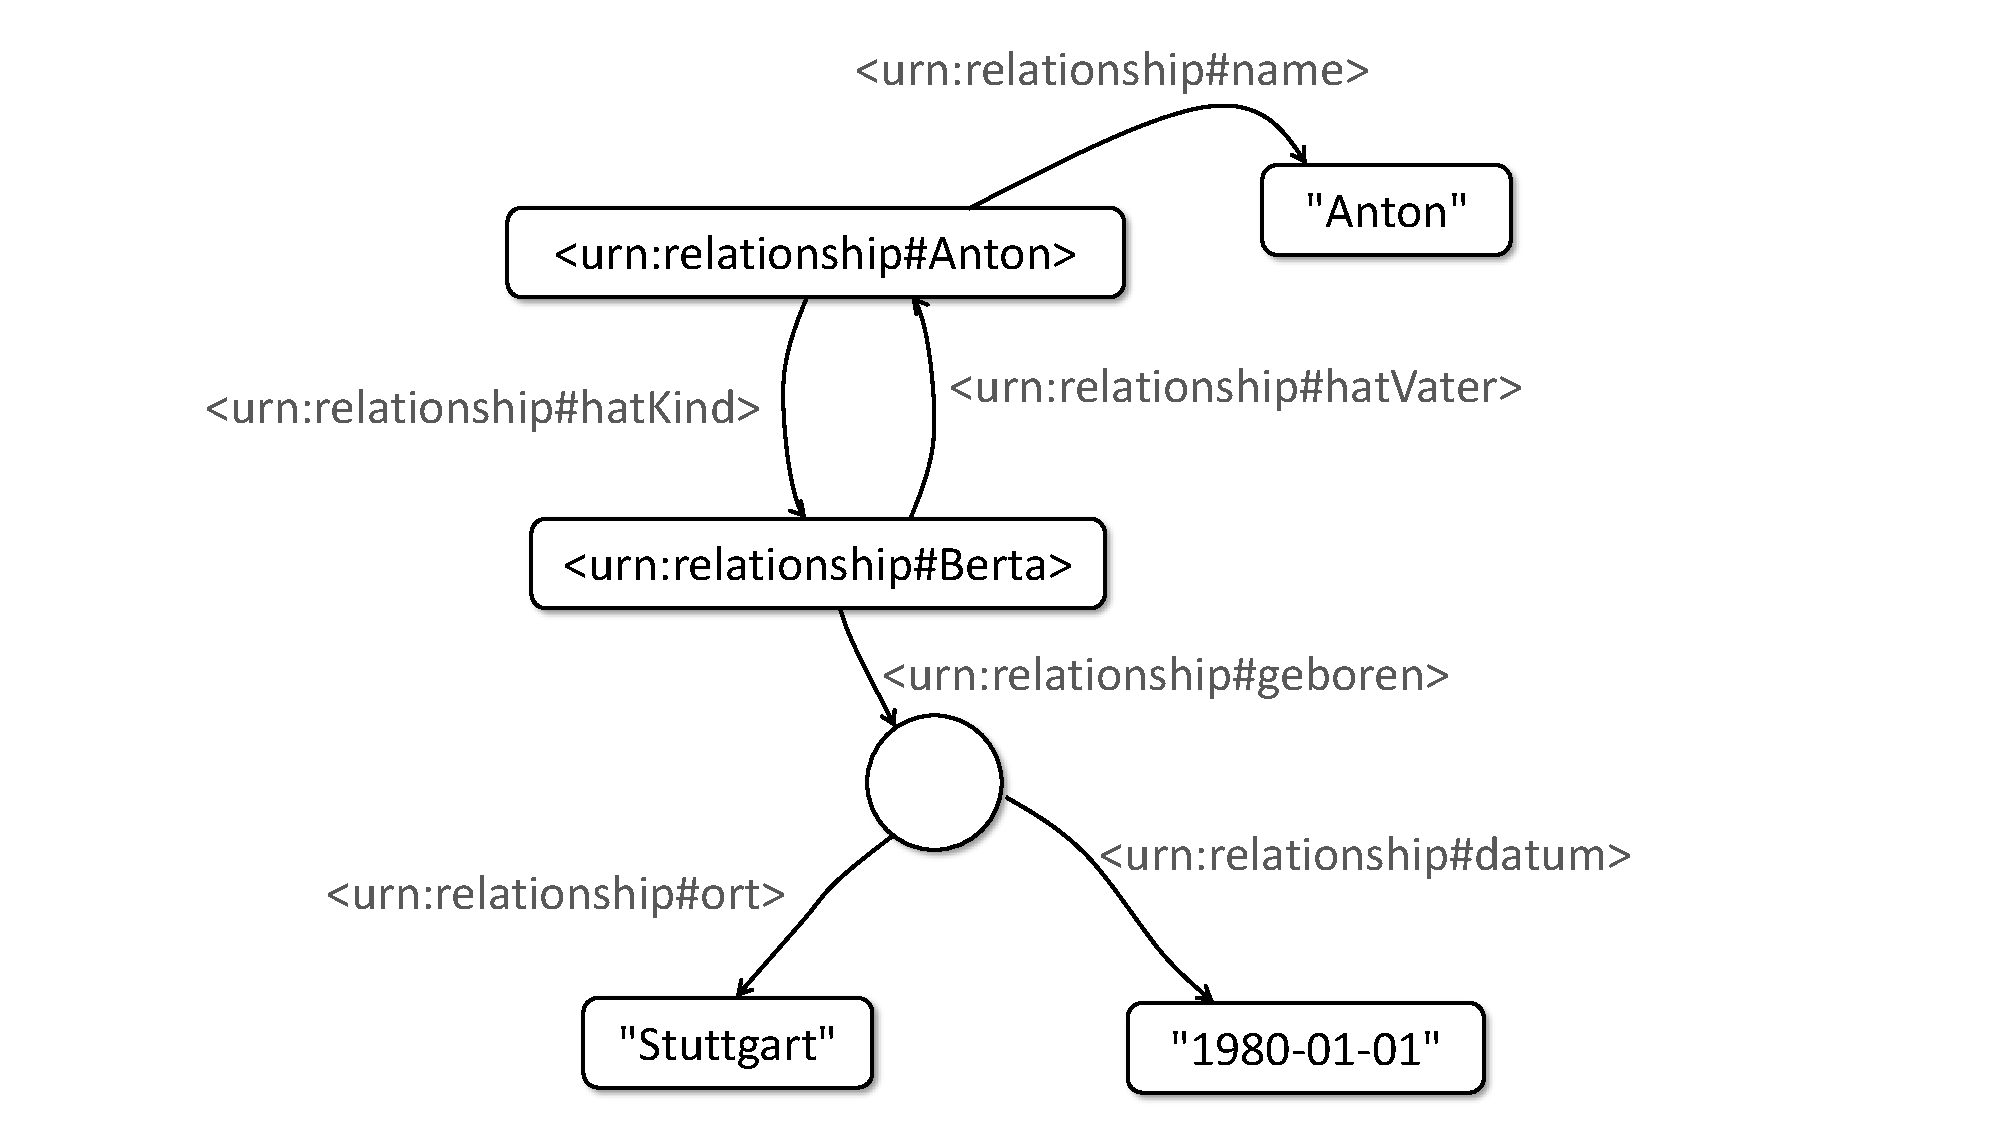
\includegraphics[width=0.7\linewidth]{resources/figures/rdfGraph}
		\caption{Visualisierung des Graphen, der von den Triples in Tabelle \ref{tab:triples} beschrieben wird. }
		\label{fig:rdfgraph}
	\end{figure}


	\subsection{RDF Syntax}

	N-Triples ist eine Syntax, bei der beliebig viele Triples hintereinander aufgelistet werden \cite[vgl.][]{w3c2014ntriples}. Die Grammatik ist in Form von regulären Ausdrücken definiert. Ein Ausschnitt davon ist in den Formeln \ref{eq:ntriple} zu sehen. Jedes n-Triples-Dokument setzt sich demnach aus abwechselnden Triples und Zeilenumbrüchen (EOL, End-Of-Line) zusammen. Ein Triple besteht aus Subjekt, Prädikat und Objekt sowie einem Punkt am Ende. N-Triples-Dateien werden mit der Dateiendung "`.nt"' versehen. Die beispielhaften Triples aus Tabelle \ref{tab:triples} sind in Quellcode \ref{lst:n-triple} dargestellt.
	\begin{align}
		\text{ntripleDoc} & ::= \text{triple?}\text{ } (\text{EOL triple})\mbox{*} \text{ EOL?} \label{eq:ntriple}\\
		\text{triple} & ::= \text{subject } \text{predicate } \text{object } \text{"'."'} \nonumber
	\end{align}
	\listingfile[caption=Beispiel einer N-Triples-Datei, label=lst:n-triple]{resources/codeSnippets/2PureTriples.ttl}
	
	Eine zweite Syntax, mit der RDF-Graphen beschrieben werden können, heißt "`Terse RDF Triple Language"' (TTL) und wird auch als "`Turtle"' bezeichnet  \cite[vgl.][]{w3c2014turtle}. Turtle-Dateien besitzen die Datei-Endung "`.ttl"'.
	Die Sprache, die von der TTL-Grammatik beschrieben wird, ist eine Obermenge der N-Triples-Sprache. Das heißt, jede gültige N-Triples-Datei ist auch eine gültige Turtle-Datei. Zusätzlich erlaubt die Turtle-Syntax weitere Schreibweisen, die es ermöglichen, Graphen übersichtlicher und mit weniger Text darzustellen. Durch syntaktische Äquivalenzumformungen lässt sich jede Turtle-Datei wieder auf eine Liste von Triples zurückführen. Somit kann jeder beliebige Graph sowohl mit N-Triples als auch mit Turtle beschrieben werden. Im Folgenden werden einige wichtige Syntax-Merkmale genauer vorgestellt.
		\paragraph{Namespaces}
		
		Die URIs in einer Datei beginnen häufig mit dem gleichen Zeichenfolge. Benannte Knoten unterscheiden sich meist nur am letzten Abschnitt des URIs. Namespaces ermöglichen, eine abgekürzte Schreibweise für URIs zu verwenden, um die Datei übersichtlicher zu machen. Ein Namespace wird mit dem Schlüsselwort \lstinline|@prefix| festgelegt, wie in Quellcode \ref{lst:ttl-namespace} zu sehen ist.
		\listingfile[caption=TTL-Datei mit Namespace, label=lst:ttl-namespace]{resources/codeSnippets/2TriplesNamespace.ttl}

		\paragraph{Liste von Prädikaten}
		Wenn in einer Turtle-Datei mehrere Triples mit dem gleichen Subjekt vorkommen, können diese Triples zusammengefasst werden. Dazu wird das erste Triple nicht mit einem Punkt, sondern mit einem Semikolon abgeschlossen. In der nächsten Zeile kommen dann nur noch Prädikate und Objekt vor. Das Subjekt wird aus der vorangegangenen Zeile wiederverwendet (siehe Quellcode \ref{lst:ttl-predicate-list}).
		\listingfile[caption=TTL-Datei mit einer Liste von Prädikaten, label=lst:ttl-predicate-list]{resources/codeSnippets/2TriplesPredicateList.ttl}

		\paragraph{Verschachtelung von Blank Nodes}
		Blank Nodes werden häufig eingesetzt, um komplexe Strukturen darzustellen. Im Beispiel setzt sich der Geburtstag aus Ort und Datum zusammen. Blank Nodes werden immer in einem bestimmten Kontext verwendet und verlieren ohne diesen Kontext ihre semantische Bedeutung. Der Knoten \lstinline|_:Geburtstag| beispielsweise ist bedeutungslos, wenn man nicht weiß, dass er zu Berta gehört. Aus diesem Grund ist es sinnvoll, dass der Knoten nicht durch einen URI auffindbar ist. Auf ihn kann nur zugegriffen werden, indem man vom Knoten Berta entlang dem Prädikat \lstinline|rel:geboren| navigiert.
		
		Auch für Blank Nodes gibt es eine Kurzschreibweise. Im Beispiel wird anstatt \lstinline|_:Geburtstag| ein Paar eckiger Klammers \lstinline|[]| geschrieben. Alle Prädikate, die von dem Blank Nodes ausgehen, werden zusammen mit dem Objekt in die eckigen Klammern geschrieben (siehe Quellcode \ref{lst:ttl-blank-node})
		\listingfile[caption=TTL-Datei mit verschachtelter Blank Node, label=lst:ttl-blank-node]{resources/codeSnippets/2TriplesBNode.ttl}

		\paragraph{RDF-Listen}
		Es gibt die Möglichkeit, von einem Knoten mehrere ausgehende Kanten zu spezifizieren, die den gleichen URN haben (siehe Quellcode \ref{lst:ttl-list} oben). Diese Modellierungmöglichkeit kann sehr einfach eingesetzt werden, aber hat den Nachteil dass die Reihenfolge der Objekte nicht spezifiziert ist. Das heißt, wenn ein Computerprogramm  die Turtle-Datei einliest, ist die Reihenfolge der Elemente zufällig bzw. abhängig von der Implementierung.
		
		Möchte man eine Liste definieren, bei der die Reihenfolge festgelegt ist, kann man RDF-Listen einsetzen (siehe Quellcode \ref{lst:ttl-list} unten). Bei der Syntax werden runde Klammern eingesetzt. Wenn Die TTL-Datei geparst wird, ist die Liste als Binärbaum dargestellt (siehe \ref{fig:rdflist}). Jeweils ein Ausgang des Knotens zeigt auf ein Listenelement, der andere Ausgang auf den Rest der Liste. Das Ende der Liste wird durch ein spezielles Objekt (rdf:nil) markiert.

\listingfile[caption=Knoten mit mehreren ausgehenden Kanten mit dem gleichen URI, label=lst:ttl-list]{resources/codeSnippets/2TriplesList.ttl}
\begin{figure}
	\centering
	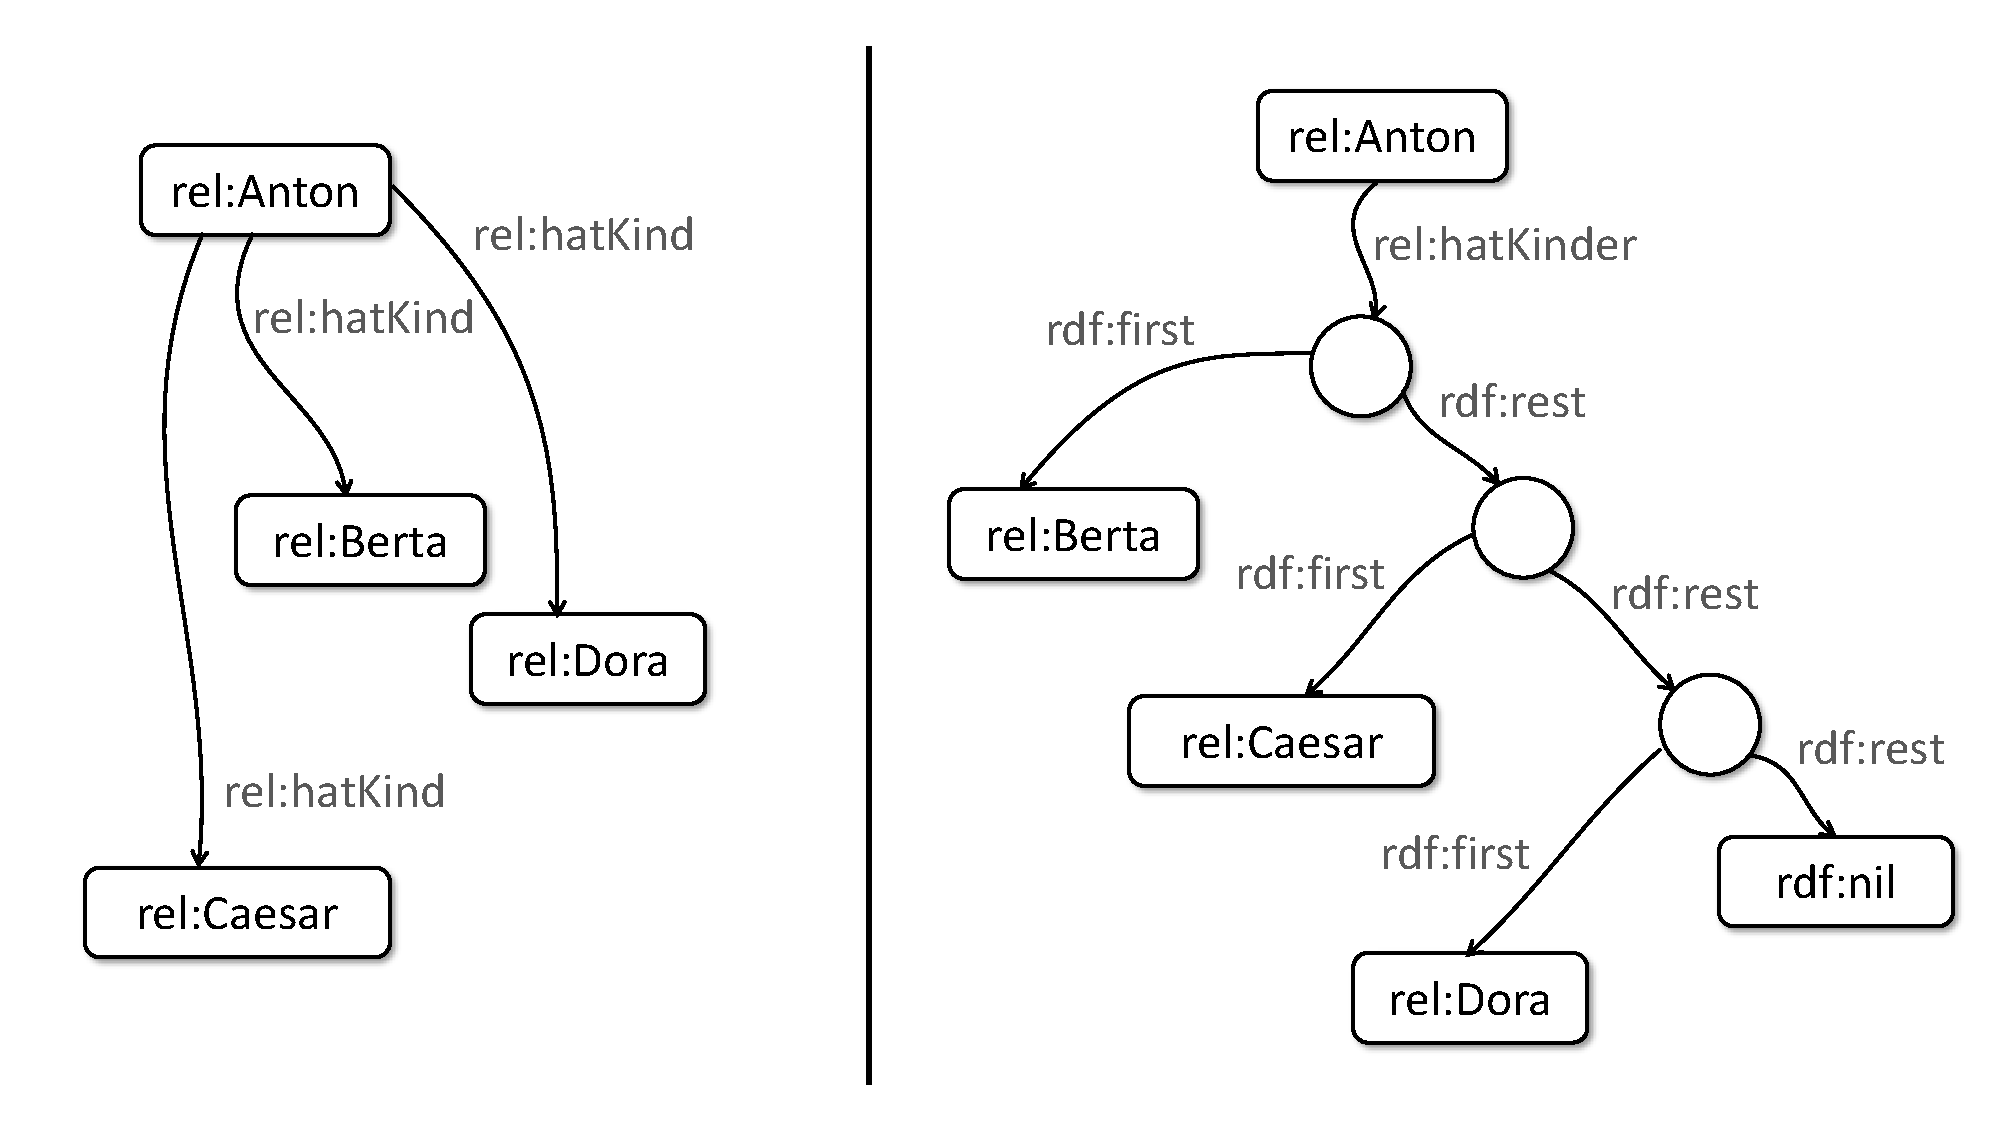
\includegraphics[width=0.7\linewidth]{resources/figures/rdfList}
	\caption[Vergleich von Merhfachverwendung eines Prädikats und RDF-Listen]{Vergleich der beiden Graphen bei mehrfacher Verwendung eines Prädikats (links) und beim Einsatz von von RDF-Listen (rechts).}
	\label{fig:rdflist}
\end{figure}

Zusammenfassend erlaubt RDF die formale Beschreibung aller möglichen Zusammenhänge. Über die Semantik, also die Bedeutung der Daten in Bezug auf die echte Welt, macht RDF keine Aussage. Die Semantik wird erst von konkreten Datenmodellen  ins Spiel gebracht, die auf RDF basieren.

\section{BAMM Aspect Meta Model (BAMM)}

Ein Metamodell ist ein Modell, das die Beschreibung von Modellen erlaubt. \cite[vgl.][S. 43f]{jeusfeld2009metamodel} Genauso wie ein Datenmodell die Struktur konkreter Daten beschreibt, so beschreibt ein Metamodell die Stuktur konkreter Modellen. Daten, Datenmodell und Metamodell bilden eine Hierarchie von drei Abstraktionsebenen.

Um Aspektmodelle zu erstellen, wird das BAMM Aspect Meta Model eingesetzt. Die Vorteile von Aspektmodellen wurden bereits in Sektion \ref{sec:aspektmodelle} genannt. In diesem Abschnitt werden die Modellierungsmöglichkeiten von Aspektmodellen beschrieben. Die Spezifikation des BAMM Aspect Meta Models setzt sich aus zwei Komponenten zusammen.
\begin{itemize}
	\item Es definiert eine Menge von Modellelement-Klassen. Beispiele solcher Klassen sind "`Aspect"', "`Property"', "`Characteristic"' oder "`Unit"'. Innerhalb von Aspektmodellen werden dann Instanzen der Klassen eingesetzt, und in Beziehung zueinander gesetzt. Die Gesamtheit mehrerer Modellelement-Instanzen und deren Verbindungen formen ein Aspektmodell.
	\item Die zweite Komponente des BAMM ist eine Menge an Regeln, die vorschreibt, wie die Instanzen der Modellelemente modelliert werden dürfen. Beispielsweise kann ein Aspekt beliebig viele Properties besitzen, aber keine Entities. Ein Aspektmodell, bei dem alle Regeln eingehalten sind, nennt man valide.
\end{itemize}

Ein dritter Teil, der vom BAMM bereitgestellt wird, ist ein Katalog an vorgefertigten Modellelement-Instanzen. Dazu gehören zum Beispiel häufig eingesetzte Datenstrukturen wie Zeitreihen oder 3D-Vektoren. Dieser Teil wäre in der Spezifikation nicht zwangsweies nötig, aber bietet Anwendern den Komfort, dass häufig eingesetzte Modellierungen nicht selbst modelliert werden müssen.

Das BAMM Aspect Meta Modell ist nicht komplett eigenständig, sondern basiert auf weitverbreitete Standards wie zum Beispiel:
\begin{itemize}
	\item Das Resource Description Framework (RDF). \cite[vgl.][]{w3c2014rdf}
	\item Standardisierte Datentypen des World Wide Web Consortiums (W3C). \cite[vgl.][]{w3c2004datatypes}
	\item Einen Katalog an physikalischen Einheiten, der von der Wirtschaftskommission UNECE empfolen wird. \cite[vgl.][]{unece2021units}
\end{itemize}

	\subsection{Modellelement-Klassen des BAMM}

	Im Folgenden wird ein Überblick über die wichtigsten Modellelemente gegeben und an Beispielen veranschaulicht. Um Inkonsistenten bei Übersetzungen zu vermeiden, werden stets die englischen Bezeichnungen gennant. Lediglich für Bezeichner mit einer ähnlichklingenden Übersetzung wird innerhalb von Sätzen die deutsche Bezeichnung verwendet, um den Lesefluss nicht zu stören.
	{\color{red} Diagramm mit Übersicht }

		\paragraph{Aspect} Die Modellelement-Klasse Aspekt ist das Wurzelelement eines Aspektmodells. Es beschreibt die bereitgestellten Daten eines Aspekt und ist somit eine Spezifikation für die Implementierung des Aspekts. Im Aspektmodell setzt sich der Aspekt aus einer Menge von Properties, Operations und Events zusammen.
		
		\paragraph{Property} Eine Property ist eine Eigenschaft, die das Objekt der echten Welt besitzt. Beispielhafte Properties sind Sensorwerte einer Maschine, die Fahrzeugidentifizierungsnummer eines Fahrzeugs oder die aktuelle Version einer installierten Software.
		
		\paragraph{Operation} Funktionalitäten, die eine Solution triggern kann, sodass das Asset diese ausführt, bezeichnet man als Operation. Operationen haben beliebig viele Eingabeargumente und einen optionalen Rückgabewert. Beispiele hierfür sind das Starten oder Stoppen einer Maschine oder das Auslesen eines Fehlerspeichers.
		
		\paragraph{Event} Ein Event ist ein einmaliges Ereignis, das zu einem bestimmten Zeitpunkt auftritt und an den Aspekt gemeldet werden sollte, damit dieser darauf reagieren kann. Für eine Maschine könnten sinnvolle Events zum Beispiel das manuelle Öffnen einer Türe sein, oder das Aufbrauchen von Rohmaterial. Events sind vor allem dann nützlich, wenn es eine Echtzeitverbindung zwischen Asset und Aspekt gibt.
		
		\paragraph{Characteristic} Eine Charakteristik beschreibt die Darstellung und den Datentyp einer Property. Wenn eine Solution und eine Aspekt wärend der Laufzeit über HHTP kommunizieren, dann werden Properties in einer JSON-Struktur dargestellt. Jede Property ist entweder ein nativer Typ (String, Zahl, boolescher Wert, Null) oder eine komplexere Struktur (Array, Objekt). Wie genau eine Property darstellt wird, spezifiziert eine Charakteristik. {\color{red} Enumeration, Collection}
		
		\paragraph{Entity} Für den Fall, dass eine Property als JSON-Objekt mit geschachtelten Werten dargestellt wird, werden Entities eingesetzt. Eine Entity ist ein Datentyp, der mehrere Unter-Properties besitzt. Um die Anwendung zu verdeutlichen, wird im Folgenden ein Beispiel dargestellt.
		
		Eine CNC-Fräsmaschine hat als Eigenschaft eine Position im dreidimensionalen Raum. Ein Aspekt soll diese Eigenschaft bereitstellen. Dafür wird im Aspektmodell eine Property mit dem Namen "`CurrentPosition"' erstellt. Die Property besitzt eine Charakteristik, die ein Entity als Datentyp festgelegt hat. Das Entity heißt "`Vector3D"' und besitzt die drei Properties "`X"', "`Y"' und "`Z"'. Für diese Properties werden dann zum Beispiel der Datentype Float festgelegt.
		
		\paragraph{Trait und Constraints}
		{\color{red} Einschränkung für Werte durch Constraints. Beispiele RangeConstraint, RegularExpressionConstraint. Wrapping durch Trait}
		\paragraph{Vererbung}

	\subsection{Beispiel eines Aspektmodells}

\section{Software Defined Vehicle}

	\subsection{Einführung}
	Software Defined Vehicle (Software-definiertes Fahrzeug) ist ein Begriff, der die Zukunftsvision des modernen Fahrzeugs beschreibt. In der Vergangenheit wurde das Fahrerlebnis vor allem durch die Hardware bestimmt. Ein gutes Auto musste eine gute Ausstattung besitzen. Heutzutage werden die Software-Komponenten im Fahrzeug immer wichtiger, zum Beispiel bei Fahrerassistenzsystemen und Komfortsystemen, wie Sprachsteuerung.
	
	In der Zukunft wird die Software einen immer größeren Anteil im Fahrzeug einnehmen. Die Software sollte nicht für jeden Fahrzeugtyp angepasst werden müssen, sondern kompatibel mit unterschiedlichen Modellen oder sogar unterschiedlichen Herstellern sein. Zusätzlich wird das Auto der Zukunft kein isoliertes System sein, sondern mit seiner Umwelt kommunizieren. . All diese Trends sind Teil des Software-definierten Fahrzeugs.
	
	\subsection{Stand der Technik}
	\subsection{Vehicle Service Specification (VSS)}

\section{Python}
	Python ist eine höhere Programmiersprache, die zur Lösung vieler unterschiedlicher Probleme eingesetzt werden kann. Die Python Software Foundation ist für die Entwicklung der Sprache zuständig \cite[vgl.][]{python2022usecases}. Im Folgenden wird ein kurzer Überblick über die Eigenschaften von Python und möglichen Anwendungsfälle gegeben.
	
	\subsection{Charakteristiken} \label{sec:py-characteristics}
		\paragraph{Interpretation statt Kompilierung} Python zeichnet sich dadurch aus, dass der Quellcode nicht kompliliert wird, sondern während der Laufzeit Instruktion für Instruktion interpretiert wird. Im Vergleich zu anderen Programmiersprachen ergeben sich dadurch Stärken und Schwächen und somit auch bestimmte Einsatzgebiete. 
		
		Um Python-Code auszuführen, benötigt man eine Implementierung der Sprache, die den Code verarbeiten kann und die Instruktionen ausführt. Solch eine Implementierung bezeichnet man als Interpreter. Genauso wie es für kompilierte Programmiersprachen häufig unterschiedliche Compiler gibt, so gibt es für Python verschiedene Interpreter. Der weitverbreitetste heißt CPython und ist in C und Python geschrieben. CPython wird von der Python Software Foundation veröffentlicht und wird als De-Facto-Standard der Sprache angesehen \cite[vgl.][S. 25]{python2014brochure} \cite{github2022cpython}.
		
		\paragraph{Performance} Ein Python-Programm ist deutlich langsamer als komplierter Code, zum Beispiel mit C++. Das liegt daran, dass Quellcode in C++ nur zum Kompilieren benutzt wird, um leichtgewichtigen Assembly-Code zu generieren. Während der Laufzeit müssen lediglich noch die Instruktionen auf der Hardware durchgeführt werden.
		Bei Python hingegen wird der Code während der Laufzeit zu Byte-Code und anschließend zu Maschinencode verarbeitet, wofür sehr viel Rechenkapazität benötigt wird. Zum Importieren anderer Python-Dateien (Module) muss der Quellcode der Ziel-Datei während der Laufzeit eingelesen und zu einem Syntax-Baum geparst werden. Auch dies benötigt sehr viel Rechenaufwand. In C++ ist kein Importieren zur Laufzeit nötig, da schon beim Komplieren und Linken all benötigten Programmteile vereinigt werden. Benchmarks zeigen, dass ein C++-Programm für rechenaufwändige Algorithmen bis zu einhundert mal so schnell terminiert. Ein allgemeingültiger Wert lässt sich jedoch nicht messen, da die Performance immer vom Algorithmus und der Implementierung abhängig ist. \cite[vgl.][]{banchmarkgame2022cpppython}
		
		\paragraph{Typisierung} Eine weitere Charakteristik von Python ist, dass es keine strenge Typisierung gibt. Während in Java oder C++ für jede Variable, jedes Eingabeargument und jeden Rückgabewert ein Typ angegeben werden muss, ist dies bei Python nicht nötig. Der Typ einer Variablen kann sich sogar durch eine Operation verändern. Anzumerken ist auch, dass Variablen nicht deklariert werden müssen bevor sie zugewiesen werden.
		
		Seit einiger Zeit ist es möglich, sogenannte "`Type Hints"' anzugeben, also Informationen darüber, welchen Typ eine Variable, ein Eingabeargument oder ein Rückgabewert besitzt. Diese dienen als Komfort zur Entwicklungszeit, da Entwicklungsumgebungen (IDEs) Autovervollständigung und ähnliches anbieten können. Während der Laufzeit eines Python-Programms werden Type Hints ignoriert.
		
		\paragraph{Syntax} Die Syntax von Python gilt als sehr gut lesbar \cite[vgl.][]{bassi2007primer}. Die Strukturierung von Codeblöcken erfolgt durch Einrückung von Zeilen. Semikolons nach Instruktionen und Klammern zur Strukturierung sind nicht nötig. Ausdrücke, in Bedingungen und Schleifen können häufig sehr intuitiv formuliert werden. 
		Im Folgenden ist ein Vergleich zwischen C- und Python-Syntax äquivalenter Ausdrücke dargestellt (siehe Quellcode \ref{lst:c-code} und \ref{lst:python}).
	
\listingfile[caption=Beispielcode in C, label=lst:c-code]{resources/codeSnippets/2CCode.c}

\listingfile[caption=Beispielcode in Python, label=lst:python]{resources/codeSnippets/2PythonCode.py}
			
		
		\paragraph{Objekte} Python bietet die Möglichkeit objektorientiert zu programmieren. Das Klassenkonzept ist ähnlich zu dem von C++ oder Java, aber unterscheidet sich bei genauerer Betrachtung.
		
		Während man in C++ und Java unter dem Begriff "`Objekt"' die Instanzen von Klassen meint, ist der Begriff in Python viel weitreichender. Genau genommen sind fast alle Datenstrukturen in Python Objekte. Dazu zählen zum Beispiel:
		\begin{itemize}
			\item \textbf{Instanzobjekte} Jedes Mal, wenn eine neue Instanz einer Klasse erstellt wird, erzeugt Python ein Objekt, das Referenzen zu allen Felder (Membervariablen) besitzt. 			
			\item \textbf{Klassenobjekte} Nicht nur Instanzen von Klassen, sondern auch Klassen selbst, sind Objekte. Für jede Klasse, die in einem Programm deklariert ist, gibt es ein Objekt im Speicher. Dieses enthält zum Beispiel Referenzen zu den Methoden und zu den statischen Feldern.
			\item \textbf{Funktionen} Eine Funktion enthält den Syntax-Baum der Python-Instruktionen und Informationen über Eingabeargumente und Rückgabewert. Jedes Funktions-Objekt besitzt eine Methode \lstinline|__call__()|, mit der die Funktion ausgeführt werden kann.
			\item \textbf{Module und Pakete} Ein Modul ist Abkapselungen von Python-Code in einer separate Datei. Ein Paket ist eine Abkapselung in einem separaten Order. Ein Modul oder Paket, das in ein Programm importiert wird, liegt als Objekt im Speicher und enthält Referenzen zu den enthaltenen Inhalten wie Klassen, Funktionen oder Untermodulen.
			\item \textbf{Builtin-Datentypen} Datentypen, die von Python mitgeliefert werden und nicht vom Entwickler selbst erstellt werden müssen, sind ebenfalls Objekte. Die Datentypen "`int"', "`str"' und "`float"' sind Klassenobjekte und die konkreten Werte wie "`10"', "`hello"' oder "`2.4"' sind Instanzobjekte.
			\item \textbf{True und False} In vielen anderen Programmiersprachen ist ein Wahrheitswert ein einfacher Wert, der als 0 oder 1 im Speicher steht. In Python gibt es die Klasse "`bool"' und davon die beiden Instanzen "`True"' und "`False"'. Die beiden Instanzen werden beim Starten des Programms erzeugt und es können keine neuen Instanzen erstellt werden.
		\end{itemize}
	\subsection{Einsatzgebiete}		
		Die Bereiche, für die Python als Programmiersprache eingesetzt wird, sind sehr breit. Gegenüber anderer Programmiersprachen ist Python einfach zu lernen. \cite[vgl.][]{saabith2019python} Des weiteren kann das selbe Problem meist in weniger Zeilen Code gelöst werden, verglichen mit anderen Programmiersprachen \cite[vgl.][S. 100]{mcconnell2009code}.
		Aus diesen Gründen, eignet sich Python vor allem dort, wo genug Performance zur Verfügung steht und mit wenig Entwicklungszeit ein großer Fortschritt erzielt werden soll.
		
		Python ist aufgrund seiner geringeren Performance nicht für Anwendungen mit wenig Rechenkapazität und kleinem Speicher geeignet, wie Steuergeräte. Für sicherheitskritische Anwendungen im Kontext eingebetteter Systeme, ist Python im Moment keine Option, da es für Python keine Standards wie MISRA gibt.
		
		Weiterhin nutzt der verbreitetste Python-Interpreter CPython zur Erstellung von Objekten den Heap. Zur Freigabe von Speicher wird ein Garbage Collector eingesetzt. Beide Eigenschaften sprechen gegen den Einsatz auf eingebetteten Systemen, da die Speicherallokation und -freigabe unkontrolliert und quasi zufällig abläuft und den Code somit kaum verifizierbar macht. Es gibt andere Python-Interpreter, die speziell für eingebettete System konzipiert sind, wie MicroPython \cite[vgl.][]{george2018micropy}. Solche angepassten Interpreter sind aktuell nicht etabliert.
		
	\subsection{Werkzeuge}
		Für viele Use-Cases gibt es Python-Bibliotheken von Drittanbietern (auch Pakete genannt), die der Entwickler nutzen kann, um Entwicklungszeit einzusparen. Viele verfügbaren Pakete sind sehr robust und haben sich als De-Facto-Standard etabliert. Einige der eingesetzten Pakete werden im Folgenden vorgestellt.
		\paragraph{Poetry} Beim Einsatz von Drittanbieter-Paketen entsteht oft eine lange Liste an Abhängigkeiten, da viele Pakete weitere Pakete benötigen. Poetry ist ein Werkzeug, das die Installation aller Abhängigkeiten in der benötigten Version übernimmt. Poetry arbeitet mit virtuellen Umgebungen, also mit einem isolierten Bereichen im Dateisystem für jedes Projekt. Dadurch ist sichergestellt, dass getrennte Projekte, die die gleichen Abhängigkeiten besitzen, nicht aufeinander einwirken. Virtuelle Umgebungen haben auch den Vorteil, dass sie unabhängig von bereits installierten Paket-Versionen sind, und somit die Verteilung auf andere Geräte erleichtern.
		
		Poetry bietet außerdem Funktionen zum Packen und Veröffentlichen von Paketen.
		\paragraph{MyPy} Wie in Sektion \ref{sec:py-characteristics} beschrieben, werden Typen von Objekten während der Laufzeit nicht geprüft. Es ist beispielsweise möglich, eine Funktion, die einen Zahlenwert fordert, mit einem String aufzurufen. Die richtige Funktion des Programms ist damit nicht mehr sichergestellt. Das Verifizieren von Software ist somit extrem schwierig, da jede Funktion darauf angewiesen ist, dass sie von anderen Funktionen richtig aufgerufen wird. MyPy ist ein Paket, das eine statische Codeanalyse durchführt und sicherstellt, dass Type Hints eingehalten werden.
		
	
\section{weitere Technologien}
	\subsection{Open API Specification}
	\subsection{Authentifizierung mit OAuth2}
	
	\chapter{Konzeption}
\fancyhfStyleContent{}
	\chapter{Implementierung}
\fancyhfStyleContent{}
	\chapter{Zusammenfassung und Ausblick}
\fancyhfStyleContent{}
	
	\setstretch{1.0}
	\printbibliography[title=Literaturverzeichnis, heading=bibintoc]

\end{document}          
